En el caso sin ruido un retraso general requiere aproximarse a una codificacion\'on ideal. Ahora tiene una 
funci\'on adicional que permite una muestra amplia de ruido para afectar a la se\~{n}al antes de cualquier juicio, se hace 
en el punto de resepci\'on para el mensaje original. Incrementando el tama\~{n}o del ejemplo siempre agudiza las
posibles afirmaciones estad\'isticas.

El contenido del teorema \ref{th:11} y su prueba se pueden formular de una manera diferente que muestra 
una conexi\'on sin ruido de una manera mas clara. Tenga en cuenta las posibles se\~{n}ales de duraci\'on T y supongamos 
que un subconjunto de ellos es seleccionado para ser usado. Los que est\'en en el subconjunto se utilizan todos con igual probabilidad, y suponiendo 
que el reseptor est\'a construido para seleccionar, como la se\~{n}al original, la causa m\'as probable del subconjutno, cuando 
una se\~{n}al perturbada es recivida. Nosotros definimos $N(T,q)$ siendo el numero m\'aximo de se\~{n}ales que podemos elegir 
para el subconjunto tal que la probabilidad de una interpretaci\'{o}n incorrecta sea menor o igual a $q$.

\begin{theorem}
\label{th:12}
  \begin{equation} \lim_{T \to{} \infty}\frac{\log{N}(T,q)}{T} =
    C, \end{equation} donde $C$ es la capacidad del canal,siempre
    que q no sea igual a 0 o 1
\end{theorem}

En otras palabras, no importa la forma en que se establece los l\'imites de fiabilidad, podemos distinguir de forma fiable mensajes 
en tiempo $T$ para corresponder a $CT$ bits, cuando $T$ es suficientemente grande. 
En el teorema \ref{t12} podemos comparar la capacidad de un canal sin ruido dado en la secci\'on uno \ref{secc:1}.

\clearpage

\chapter{Ejemplo de un canal discreto y su capacidad}
\label{sec:15}

Un ejemplo simple de un canal discreto se indica en la figura \ref{fig:11}. Hay tres posibles s\'imbolos. El primero nunca se
vera afectado por el ruido. El segundo y el tercero tienen cada uno una probabilidad $p$ de llegar inalterado y 
$q$ de ser cambiado en otro elemento par. Tenemos (permitiendo $\alpha = -[p \log p + q\log{q}]$ y $P$ y $Q$ son 
probabilidades de estar usando los s\'imbolos primero y segundo).

\begin{figure}[!ht]
\centerline{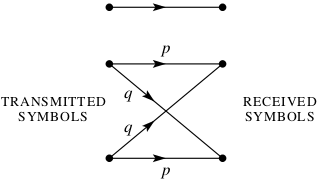
\includegraphics[width=80mm]{Imagenes/SinComentarios/Pagina25-Figura11.png}}
\caption{Un ejemplo de un canal discreto.}
\label{fig:11}
\end{figure}

\begin{equation}
\begin{array}{rcl}
H(x) &=& -P\log{P} - 2Q\log{Q} \\
H_y(x) &=& 2Q\alpha
\end{array}
\end{equation}

Nosotros deseamos elegir $P$ y $Q$, de tal manera que se maximice
$H(x) - H_y(x)$ sujeto a la restricci\'on $P + 2Q = 1$.

Por lo tanto consideremos:
\begingroup
\renewcommand*{\arraystretch}{2.0}
\begin{equation}
\begin{array}{rcl}
U &=& -P\log{P} - 2Q\log{Q} -2Q\alpha + \lambda(P+2Q) \\
\displaystyle\frac{{\partial U}}{{\partial P}} &=& -1 - \log{P} + \lambda = 0 \\
\displaystyle\frac{{\partial U}}{{\partial P}} &=& -2 - 2\log{Q} -2\alpha + 2\lambda = 0
\end{array}
\end{equation}
\endgroup

Eliminando $\lambda$
\begin{equation}
\begin{array}{rcl}
\log{P} &=& \log{Q} + \alpha \\
P &=& Q e^\alpha = Q\beta 
\end{array}
\end{equation}

\begin{equation}
  P = \frac{\beta}{\beta + 2} \\ 
  Q = \frac{1}{\beta + 2}
\end{equation}

La capacidad del canal es de:

\begin{equation}
  C = \log{\frac{\beta + 2}{\beta}}
\end{equation}

N\'{o}tese como esto comprueba los valores obvios en los casos: $p =
1$ y $p = \frac{1}{2}$. En primero, $\beta = 1$ y $C = \log{3}$, el
cual es correcto debido a que el canal es entonces sin ruido con tres
posibles s\'imbolos. Si $p = \frac{1}{2}$, $\beta = 2$ y $C
= \log{2}$. Aqu\'i el segundo y el tercer s\'imbolo, no se puede
distinguir en absoluto y act\'uan conjuntamente como un solo
s\'imbolo. El primer s\'imbolo se utiliza con una probabilidad $P
= \frac{1}{2}$ y el segundo junto al tercero con probabilidad
$\frac{1}{2}$. Esto puede ser distribuido entre ellos de cualquier
modo deseado y todav\'ia alcanzar la m\'axima capacidad.  Para los
valores intermedios de la capacidad del canal $p$ estara entre
$\log{2}$ y $\log{3}$. Esta distinci\'on entre el segundo y tercer
s\'imbolo transmite alguna informaci\'on, pero no tanto como en el
caso sin ruido.  El primer s\'imbolo se utiliza tanto mas
frecuentemente que los otros dos, debido a su ausencia de ruido.

\clearpage

\chapter{La capacidad del canal en ciertos casos especiales}
\label{sec:16}

Si el ruido afecta s\'imbolos sucesivos del canal de forma
independiente pueden ser descritos por un conjunto de transici\'on de
probabilidades $p_{i,j}$. Esta es la probabilidad, si el simbolo $i$ es
enviado, que $j$ ser\'{a} recibido. La tasa de canal m\'aximo viene dado
por el m\'aximo de:

\begin{equation}
  \sum_{i,j}P_i p_{i,j} \log{\sum{P_i p_{i,j}}} + \sum_{i,j}P_i p_{i,j}\log{p_{i,j}}
\end{equation}
 
Donde variamos $P_i$ sujeto a $ \sum P_i = 1$. Esto se conduce por el m\'etodo de Lagrange para las ecuaciones,

\begin{equation}
\sum_{j}P_{sj} \log{\frac{P_{sj}}{\sum_{i} P_i p_{ij} }} = u \\
s = 1,2,....
\end{equation}

Multiplicando por $P_s$ y sumando en $s$ muestra que $\mu = C$. Se hace la inversa de $p_{sj}$ (si existe) en $h_{st}$  de modo que 
$\sum_{s}$ $h_{st}$ $p_{sj} = \delta_{tj}$. Entonces: 

\begin{equation}
  \sum_{s,j}h_{st} p_{s,j} \log{p_{s.j}} - \log{\sum_{i}P_i p_{i,t}} = C \sum_{s} h_{s,t}.
\end{equation}
Por lo tanto:
\begin{equation}
  \sum_{i} P_i p_{i,t} = \exp[- C \sum_{s} h_{s,t}+ \sum_{s,j} h_{s,t} p_{s,j} \log{p_{s,j}}]
\end{equation}
o  
\begin{equation}
  P_i = \sum_{t} h_{i,t} \exp[ - C \sum_{s} h_{s,t}+ \sum_{s,j} h_{s,t} p_{s,j} \log{p_{s,j}} ].
\end{equation}

Este es el sistema de ecuaciones para determinar el valor m\'aximo de
$P_i$, con $C$ se determina de manera que $\sum P_i = 1$. Cuando esto
est\'{a} hecho, $C$ sera la capacidad del canal y $P_i$ las
probabilidades para los s\'imbolos del canal para lograr esta
capacidad.  Si cada s\'imbolo de entrada tiene el mismo conjunto de
probabilidades en las l\'ineas que emergen de esto y lo mismo sucede a
cada s\'imbolo de salida, la capacidad puede ser calculada
f\'acilmente. Los ejemplos se muestran en la figura 12 \ref{fig:12}.
En tal caso $H_x (y)$ es independiente de la distribuci\'on de
probabilidades de los s\'imbolos de entrada, y esta dada por $-\sum
p_i \log{p_i}$. Cuando $p_i$ son los valores de probabilidad de
transici\'on de cualquier s\'imbolo de entrada. La capacidad del canal
es:

\begin{equation}
  \max [H(y) - H_x(y)] = \max H(y) + \sum p_i \log{p_i}.
\end{equation}

El valor m\'aximo de $H(y)$ es claramente  $\log{m}$ donde $m$ es el numero de s\'imbolos de salida, ya que es posible que se den 
igualmente probables haciendo los s\'imbolos de entradas igualmente probables. La capacidad del canal es por lo tanto
\begin{equation}
  C = \log{m} + \sum p_i \log{p_i}.
\end{equation}

\begin{figure}[!ht]
\centerline{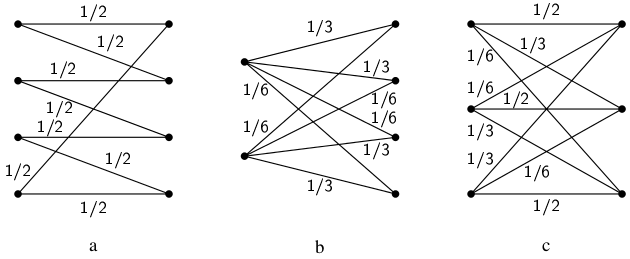
\includegraphics[width=80mm]{Imagenes/SinComentarios/Pagina27-Figura12.png}}
\caption{Ejemplos de canales discretos con las mismas probabilidades de
 transici\'{o}n para cada entrada y cada salida.}
\label{fig:12}
\end{figure}


En la figura 12a \ref{fig:12} ser\'ia
\begin{equation}
  C =  \log{4} - \log{2} 0 \log{2}.
\end{equation}
Esto se podr\'ia lograr mediante el uso solo el primer y el tercer
s\'{\i}mbolo. En la Figura 12b\ref{fig:12}:
\begin{equation}
  C = \log{4} - \frac{2}{3}\log{3} - \frac{1}{3}\log{6}
  = \log{4} - \log{3} - \frac{1}{3}\log{2}
  = \log{\frac{1}{3}} 2^{\frac{5}{3}}
\end{equation}
En la figura 12c \ref{fig:12} tenemos:
\begin{equation}
  C = \log{3} - \frac{1}{2}\log{2} - \frac{1}{3}\log{3} - \frac{1}{6} \log{6} \\
  = \log  {\frac{3}{ 2^{\frac{1}{2}} 3^{\frac{1}{3} 6^{\frac{1}{6} }}}}.
\end{equation}

Supongamos que los s\'imbolos se dividen en varios grupos tal que el
ruido causa a un s\'imbolo en un grupo a ser confundido con un
s\'imbolo de otro grupo. Deja la capacidad de un grupo n-\'esimo ser
$C_n$ (en bits por segundo) donde solo utilizamos los s\'imbolos de
este grupo. Entonces es f\'acil desmotrar que para un mejor uso de todo el conjunto, la
probabilidad $P_n$ total de todos los s\'imbolos del grupo $n$-\'{e}esimo
deber\'ia ser:

\begin{equation}
  P_n = \frac{2^{C_n}}{\sum 2^{C_n}}
\end{equation}

En un grupo la probabilidad se distribuye tal como ser\'ia si estos eran los \'unicos s\'imbolos que se utilizan. 
La capacidad del canal es:
\begin{equation}
  C = \log{\sum 2^{C_n}}.
\end{equation}

\clearpage

\chapter{Un ejemplo de codificaci\'on eficiente}
\label{sec:17}

El siguiente ejemplo, aunque es un poco irealista, es un caso en que la
coincidencia exacta para un canal con ruido, es posible. Hay dos
s\'imbolos de canal $0$ y $1$, y el ruido les afecta en bloques de siete
s\'imbolos.  Un bloque de siete o se transmite sin error, o
exactamente un s\'imbolo de los siete es incorrecta.Estas ocho
posibilidades son igualmente probables. Tenemos:

\begin{equation}
C = \max [ H(y) - H_x(y) ]
= \frac{1}{7}[7 + \frac{8}{8}\log{\frac{1}{8}}]
= \frac{4}{7} \text{ bits}/\text{s\'{\i}mbolos}
\end{equation}
Un c\'odigo eficiente, permite la correci\'on de todos los errores y
transmitir a la tasa $C$, es el siguiente (encontrado por un m\'etodo
de R.\ Hamming):
